\documentclass{article}

\usepackage{polski}
% skomentowana dla MAC wersja {inputenc}
 \usepackage[utf8]{inputenc}
% \usepackage[T1]{fontenc}
%\usepackage[cp1250]{inputenc}
\usepackage{polski}
\usepackage{amssymb}
\usepackage{color}
\usepackage{amsmath}
\usepackage{Sweave}
\usepackage{enumerate}
\usepackage{hyperref}

\title{Wpisz tutaj tytuł swojego projektu}
\author{\textbf{indeks, Imię NAZWISKO}, czwartek $11^{30}$\\ 
\textit{AGH, Wydział Informatyki Elektroniki i Telekomunikacji}\\
\textit{Rachunek prawdopodobieństwa i statystyka 2020/2021}}
\date{Kraków, \today}


\begin{document}
\Sconcordance{concordance:Untitled.tex:Untitled.Rnw:%
1 21 1 1 34 36 1 1 4 1 2 42 1 1 4 1 2 7 1 1 2 1 0 2 1 6 0 1 2 5 1 1 4 1 %
2 4 1 1 2 1 0 2 1 6 0 1 2 5 1 1 2 8 0 1 2 33 1 1 3 2 0 1 1 6 0 1 2 1 1 %
1 2 7 0 1 2 1 1 1 2 7 0 1 2 1 1 1 2 6 0 1 1 5 0 1 1 5 0 1 1 6 0 1 2 5 1 %
1 4 1 2 3 1 1 6 1 2 3 1 1 5 1 2 9 1 1 2 8 0 1 2 2 1 1 4 4 0 2 2 4 0 1 2 %
1 1 1 2 4 0 1 2 1 1 1 2 3 0 1 1 2 0 1 1 2 0 1 1 3 0 1 2 4 1 1 4 1 2 3 1 %
1 4 1 2 3 1 1 5 1 2 8 1 1 5 8 0 1 2 5 1 2 2 8 1 1 4 1 2 7 1 1 2 10 0 1 %
2 2 1 1 4 4 0 2 2 4 0 1 2 1 1 1 2 4 0 1 2 1 1 1 2 3 0 1 1 2 0 1 1 2 0 1 %
1 3 0 1 2 4 1 1 4 1 2 3 1 1 4 1 2 3 1 1 5 1 2 38 1 1 2 10 0 1 2 5 1 1 5 %
19 0 1 2 4 1 2 2 5 1 1 2 1 0 1 1 3 0 1 2 3 1 1 6 1 2 7 1 1 3 2 0 1 1 15 %
0 1 2 16 1 1 2 16 0 1 2 13 1 1 2 1 0 8 1 7 0 1 2 5 1 1 2 1 3 3 1 2 2 12 %
1 1 7 1 2 9 1 1 4 1 2 8 1 1 4 1 2 7 1 1 5 1 2 5 1 1 4 1 2 15 1 1 4 1 2 %
8 1 1 4 1 2 3 1 1 2 7 0 1 2 5 1 1 2 1 0 1 1 3 0 1 2 9 1 1 2 1 0 1 1 26 %
0 1 2 57 1 1 2 1 0 1 1 24 0 1 2 4 1 1 2 1 0 2 1 4 0 1 2 11 1 1 3 2 0 1 %
1 17 0 1 2 2 1 1 2 1 0 1 1 26 0 1 2 12 1 1 5 3 0 1 1 4 0 1 2 23 1 1 2 1 %
3 3 1 1 2 1 3 3 1 1 2 1 3 4 1 1 2 1 3 7 1 1 3 2 0 1 1 27 0 1 2 1 1 1 4 %
1 2 4 1 1 2 1 3 3 1 1 2 1 3 3 1 1 2 1 3 4 1 1 2 1 3 25 1}

\maketitle

\textit{Ja, niżej podpisany(na) własnoręcznym podpisem deklaruję, że przygotowałem(łam) przedstawiony do oceny projekt samodzielnie i żadna jego część nie jest kopią pracy innej osoby.}
\begin{flushright}
{............................................}
\end{flushright}

\section{Streszczenie raportu}
Raport powstał w oparciu o analizę danych dotyczących ...

\section{Opis danych}
Dane do projektu pochodzą ze strony \href{url}{\texttt{http://www.stooq.pl}}. Są one ...

\section{Analiza danych}
Poniżej zamieszczono przykładowe wywołania prostych formuł z pakietu R, których składnia może przydać się w projekcie.
\subsection{Wydobywanie podstawowych informacji z danych}
Działania na liczbach, wartości funkcji w punkcie, zaokrąglanie, działania logiczne.
\begin{Schunk}
\begin{Sinput}
> 5+7
\end{Sinput}
\begin{Soutput}
[1] 12
\end{Soutput}
\begin{Sinput}
> 3*4
\end{Sinput}
\begin{Soutput}
[1] 12
\end{Soutput}
\end{Schunk}
\subsection{Estymatory przedziałowe}
Możemy też rysować, np. wykres funkcji $f(x)=2x+2$ oraz $g(x)=x^2$.
\begin{Schunk}
\begin{Sinput}
> f = function(x){2*x+2}
> g = function(x){x**2}
> curve(f, from=-1, to=10, xlab="argumenty", ylab="wartosci", col="red")
> curve(g, from=-1, to=10, xlab="x", ylab="y", col="blue", lwd=4, add=TRUE)
\end{Sinput}
\end{Schunk}
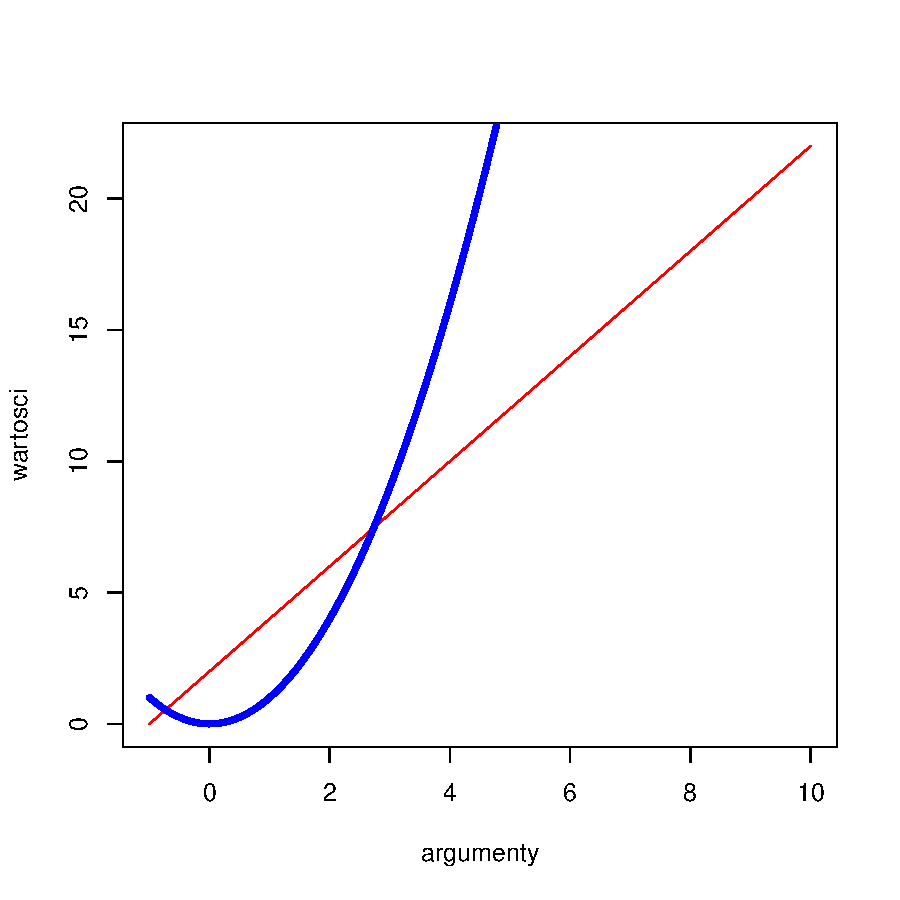
\includegraphics{Untitled-wykresyfg}

Równie dobrze można narysować gęstość rozkłądu normalnego standardowego.
\begin{Schunk}
\begin{Sinput}
> curve(dnorm(x,0,1), from=-4, to=4, xlab="x", ylab="f(x)", col="green", lwd=2)
> abline(h=0.2,col="red")
\end{Sinput}
\end{Schunk}
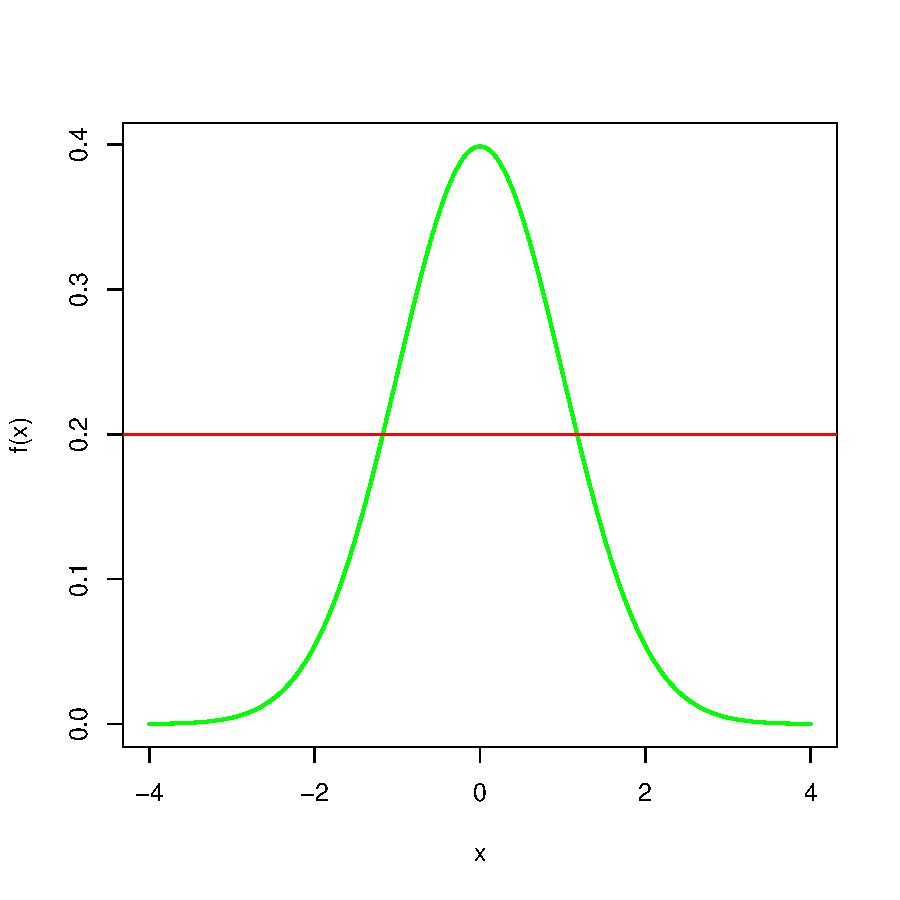
\includegraphics{Untitled-wykresyNORM}

\subsection{Testowanie hipotez}
Testować będziemy hipotezę zerową {\bf{H0}}: ... wobec hipotezy alternatywnej {\bf{H1}}: ...
Korzystam ze statystyki $t$-Studenta postaci
\begin{align*}
t=\sum_{i=1}^n\frac{licznik X_i}{mianownik^2}
\end{align*}

\subsection{Regresja}

W ten sposób można zapisać równania w \LaTeX, znakiem AND wyrównujemy je, a dwa slashe służą do przejścia do kolejnej linii.
\begin{align*}
y&=a\cdot x+b+\varepsilon,\\
z&=3\cdot y.
\end{align*}

\section{Wnioski}
Wnioski płynące z przeprowadzonej analizy, są następujące:
\begin{itemize}
\item wniosek pierwszy,
\item wniosek drugi,
\item i kolejne.
\end{itemize}

\end{document}
